\documentclass[12pt,letterpaper]{article}

\usepackage[margin=0.72in,top=0.62in,bottom=0.62in]{geometry}
\usepackage{amsmath,amssymb}
\usepackage{enumitem}
\usepackage{hyperref}
\usepackage[dvipsnames]{xcolor}
\usepackage{microtype}
\usepackage{parskip}
\usepackage{titlesec}
\usepackage{booktabs}
\usepackage{graphicx}
\usepackage{array}
\usepackage{tikz}
\usetikzlibrary{arrows.meta,positioning}

\hypersetup{
  colorlinks=true,
  linkcolor=NavyBlue,
  citecolor=NavyBlue,
  urlcolor=NavyBlue
}

\titleformat{\section}{\large\bfseries}{\thesection}{1em}{}
\titleformat{\subsection}{\normalsize\bfseries}{\thesubsection}{1em}{}
\setlength{\parskip}{0.24em}
\setlength{\textfloatsep}{10pt plus 2pt minus 2pt}
\setlength{\intextsep}{8pt plus 2pt minus 2pt}
\setlength{\abovecaptionskip}{4pt}
\setlength{\belowcaptionskip}{0pt}

\begin{document}

\begin{center}
{\LARGE\bfseries Cross-Patient Neural Speech Decoding\\[4pt]
via Atlas-Guided Spatial Calibration}\\[12pt]
{\normalsize Ben Tang \quad\textbar\quad Cogan Lab, Duke University \quad\textbar\quad April 2026}
\end{center}

\smallskip\noindent\rule{\textwidth}{0.4pt}\smallskip


%% ====================================================================
\section{The Problem}
%% ====================================================================

Cross-patient speech decoding fails for a simple reason: patients do \textbf{not} share an electrode space.

Each patient has a 128- or 256-channel $\mu$ECoG array placed by the surgeon on ventral sensorimotor cortex during intra-operative speech. Arrays differ in position, rotation, and coverage. Channel~17 in one patient is not the same brain location as channel~17 in another. Across patients, array centroids are offset by tens of millimeters, so a cross-patient model cannot rely on channel identity or grid position.

The problem is therefore: decode speech only after mapping different electrode layouts into the same functional space.


%% ====================================================================
\section{The Core Idea}
%% ====================================================================

The architecture separates cross-patient decoding into two problems:

\begin{enumerate}[leftmargin=2em, itemsep=0.15em]
\item \textbf{Spatial calibration} (per-patient): map each patient's electrodes into a common set of 16 cortical regions.
\item \textbf{Shared dynamics} (across patients): decode phoneme sequences from that common regional representation.
\end{enumerate}

This gives a clean interface:
\[
\text{electrodes} \;\longrightarrow\; \text{16 regional activations} \;\longrightarrow\; \text{phoneme sequence}
\]

The claim is not that patients share an electrode layout. The claim is that they share a \textbf{regional organization for speech}, and that the atlas gives a strong enough prior to calibrate each patient's partial observation into that common space.


%% ====================================================================
\section{Why This Should Work}
%% ====================================================================

\textbf{Speech cortex has conserved large-scale organization.} Face, tongue, sensory, Broca's, and auditory regions occupy a consistent order even though their exact coordinates vary across individuals.

\textbf{Field potentials are geometry-driven mixtures.} High-gamma at an electrode reflects nearby cortical activity weighted by distance, so the mapping is primarily geometric.

\textbf{The atlas gives the right prior.} Brainnetome provides anatomically meaningful speech-relevant regions rather than anonymous learned tokens. In a 10-patient regime, that prior matters.

\begin{figure}[ht]
\centering

\includegraphics[width=0.42\textwidth]{figures/brainnetome_parcellations_surface.png}
\caption{Brainnetome parcellation probabilities projected to the left fsaverage surface. Colors mark the 16 active speech-relevant regions; faint gray points show pooled patient electrode coverage.}
\end{figure}


%% ====================================================================
\section{Model in One Picture}
%% ====================================================================

\begin{center}
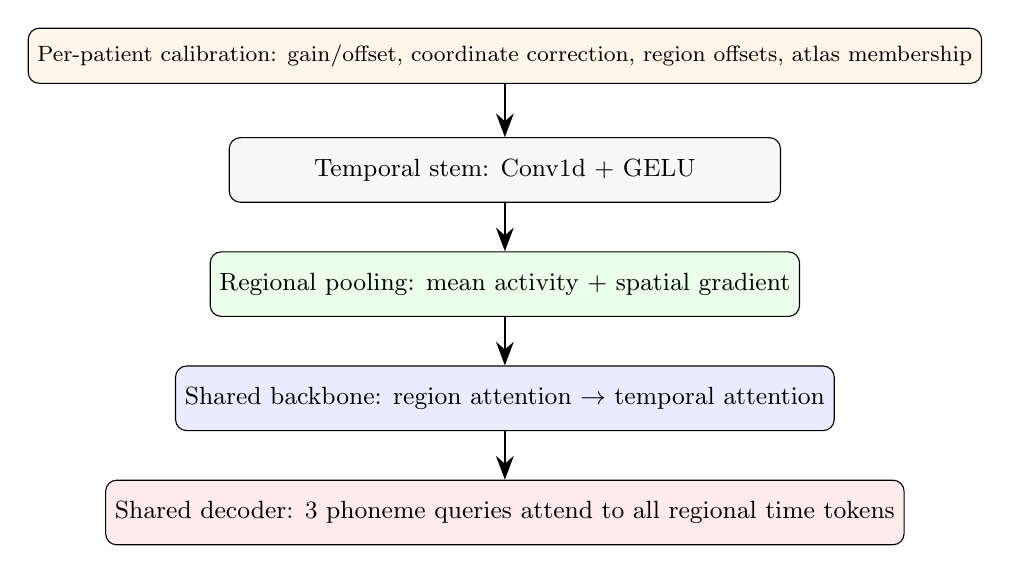
\begin{tikzpicture}[
  box/.style={draw, rounded corners, minimum width=7.0cm, minimum height=0.82cm, align=center, font=\small},
  smallbox/.style={draw, rounded corners, minimum width=7.0cm, minimum height=0.70cm, align=center, font=\footnotesize},
  arrow/.style={-{Stealth[length=3mm]}, thick}
]

\node[smallbox, fill=orange!8] (calib) at (0, 3.4) {Per-patient calibration: gain/offset, coordinate correction, region offsets, atlas membership};
\node[box, fill=gray!6] (conv) at (0, 1.95) {Temporal stem: Conv1d + GELU};
\node[box, fill=green!8] (pool) at (0, 0.5) {Regional pooling: mean activity + spatial gradient};
\node[box, fill=blue!8] (backbone) at (0, -0.95) {Shared backbone: region attention $\rightarrow$ temporal attention};
\node[box, fill=red!8] (dec) at (0, -2.4) {Shared decoder: 3 phoneme queries attend to all regional time tokens};

\draw[arrow] (calib) -- (conv);
\draw[arrow] (conv) -- (pool);
\draw[arrow] (pool) -- (backbone);
\draw[arrow] (backbone) -- (dec);
\end{tikzpicture}
\end{center}

Every patient first gets a small calibration layer that says where their electrodes sit relative to the atlas. After that, the model is shared.


%% ====================================================================
\section{Problem 1: Spatial Calibration}
%% ====================================================================

Spatial calibration is a \textbf{template-fitting problem}. The atlas provides the template; patient-specific parameters make bounded corrections.

\textbf{Signal calibration.} Each channel gets a learned gain and offset so the shared model sees comparable amplitudes across patients.

\textbf{Global coordinate correction.} A small rigid correction absorbs systematic error from surgical reconstruction and the linear MNI transform.

\textbf{Region adaptation.} Each of the 16 atlas regions gets a small patient-specific offset and a scalar temperature.

\textbf{Volumetric membership.} Electrodes are mapped to regions using Brainnetome parcellation volumes, not spherical kernels.

After calibration, every patient is represented in the same 16-region frame.


%% ====================================================================
\section{Problem 2: Shared Dynamics}
%% ====================================================================

Once the data is in a common regional space, the rest of the problem is to learn the shared dynamics that map regional activity to phoneme sequence.

\textbf{Temporal stem.} A small Conv1d converts each calibrated electrode trace into a feature sequence.

\textbf{Regional pooling.} Electrode features are compressed into 16 regional signals using average activity plus a first spatial gradient.

\textbf{Shared backbone.} Attention first models interactions across regions, then dynamics across time. This is where cross-patient sharing happens.

\textbf{Shared decoder.} Three learned queries read out the 3 phoneme positions by attending jointly across all regions and time steps.


%% ====================================================================
\section{What Is Learned Per Patient vs Shared}
%% ====================================================================

\begin{table}[ht]\centering\small
\begin{tabular}{@{}>{\raggedright\arraybackslash}p{5.4cm}>{\raggedright\arraybackslash}p{2.3cm}>{\raggedright\arraybackslash}p{5.0cm}@{}}
\toprule
\textbf{Component} & \textbf{Shared?} & \textbf{Role} \\
\midrule
Gain / offset, coordinate correction, region offsets, region temperatures & No & Calibrate where this patient's signals land in the atlas space \\
Temporal stem, regional pooling weights, spatiotemporal backbone, decoder & Yes & Learn what speech dynamics look like once signals are aligned \\
\midrule
Per-patient parameters & 326 (128-ch) & Small calibration layer \\
Shared parameters & ${\sim}$143K & One common speech decoder across patients \\
\bottomrule
\end{tabular}
\end{table}

Per-patient parameters learn \textbf{where} speech information lives in this patient. Shared parameters learn \textbf{what} that aligned activity means.


%% ====================================================================
\section{Key Risks / Decisive Tests}
%% ====================================================================

\textbf{Nonlinear MNI normalization.} The current coordinate pipeline is still linear.

\textbf{Atlas quality.} We are using smoothed atlas maps as the working representation.

\textbf{Decisive tests.} The architecture stands or falls on a few comparisons:
\begin{itemize}[leftmargin=2em, itemsep=0.1em]
\item atlas regions vs learned bottleneck
\item parcellation pooling vs cross-attention routing
\item fixed atlas vs patient-specific region offsets
\item pooled readout vs joint cross-attention decoder
\end{itemize}


%% ====================================================================
\section{Immediate Next Steps}
%% ====================================================================

\begin{enumerate}[leftmargin=2em, itemsep=0.15em]
\item \textbf{Implement the first cross-patient training loop.}
\item \textbf{Improve spatial accuracy.} If T1 MRIs are available, nonlinear MNI normalization should reduce the burden on the calibration layer.
\item \textbf{Scale shared dynamics with more data.} External chronic ECoG is most useful for pretraining the shared dynamics module, not for replacing atlas-guided calibration.
\end{enumerate}


\end{document}
